% !TEX root = 00_tcc.tex
\clearpage

\section{Estudo de Caso}

Os dados avaliados possuíam considerável quantidade de \acrshort{nan}s, como
exposto na Tabela~\ref{tbl:nan}. Para evitar o comprometimento do modelo a ser
treinado, o período dos 3 primeiros meses de 2013 foram escolhidos para servir
de dado de entrada.  O período for composto dos 3 primeiros meses do ano. Os
dados foram separados em grupos: treinamento com 75\% e teste com 25\% do total.
Dessa forma, foram 2 meses para treinamento do modelo e 1 para teste.

% !TEX root = ../0_tcc.tex

\begin{table}[ht]
	\centering
	\caption{Quantidade de \acrshort{nan}s}\label{tbl:nan}
	\begin{tabular}{lrr}
		\hline
		Data & WS\_10m &     GHI \\
		\hline
		\hline
		2006 &       0 &       0 \\
		2007 &   58185 &   58185 \\
		2008 &  137714 &  137714 \\
		2009 &   26791 &   26791 \\
		2010 &    5651 &    5651 \\
		2011 &    3120 &    3120 \\
		2012 &   38798 &   38798 \\
		2013 &    5520 &   11269 \\
		2014 &       3 &    2106 \\
		2015 &   10278 &   39468 \\
		2016 &   13380 &   21841 \\
		2017 &  126826 &  126826 \\
		\hline
	\end{tabular}
\end{table}


A velocidade do vento no local foi insuficiente para manter a operação da
aerogerador por longos períodos, devido a sua velocidade de \emph{cut-in}. O
histograma da Figura~\ref{fig:hist} mostra a frequência da velocidade corrigida
pela Equação~\ref{eq:wind:pl} para uma altura de 35 metros. Percebe-se que a
maioria encontra-se ao redor de 4 $m/s$, próximo ao começo de operação.

\begin{figure}[ht]
	\centering
	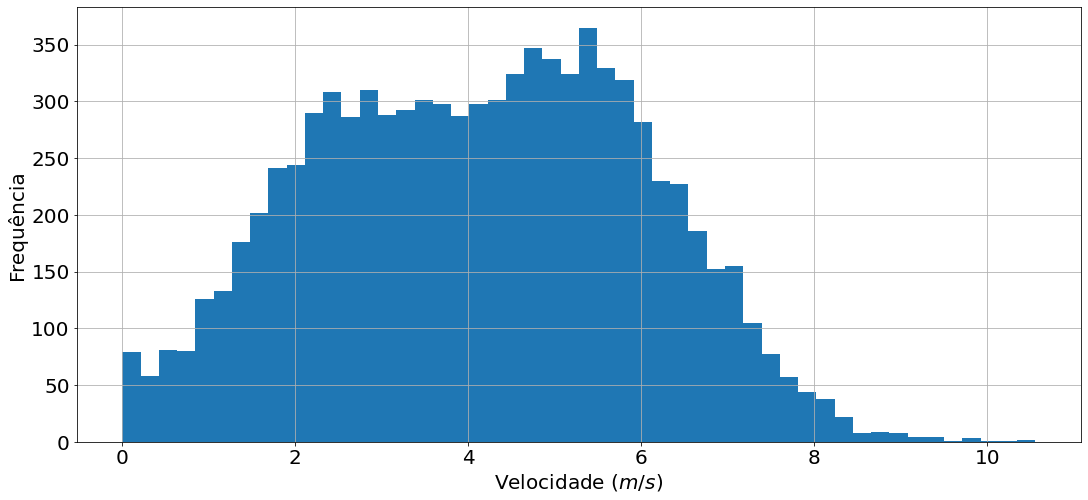
\includegraphics[width=0.8\textwidth]{../img/wind_hist.png}
	\caption{Histograma da velocidade do vento}\label{fig:hist}
\end{figure}

\subsection{Resultados}

O treinamento das redes atingiu baixos valores de \acrshort{rmse}, permanecendo
na segunda casa decimal, em parte por causa da normalização da
Equação~\ref{eq:minmax}. Ficou perceptível que a medida em que tenta-se realizar
predições de mais longo prazo, o desempenho diminui, como exposto na
Figura~\ref{fig:rmse}. Na figura, a linha laranja, com legenda de
\acrshort{ghi}\footnote{\acrlong{ghi}}, representa as redes de previsão solar. A
linha azul, \acrshort{ws10m}\footnote{\acrlong{ws10m}}, representa as redes de
previsão eólica.

\begin{figure}[ht]
	\centering
	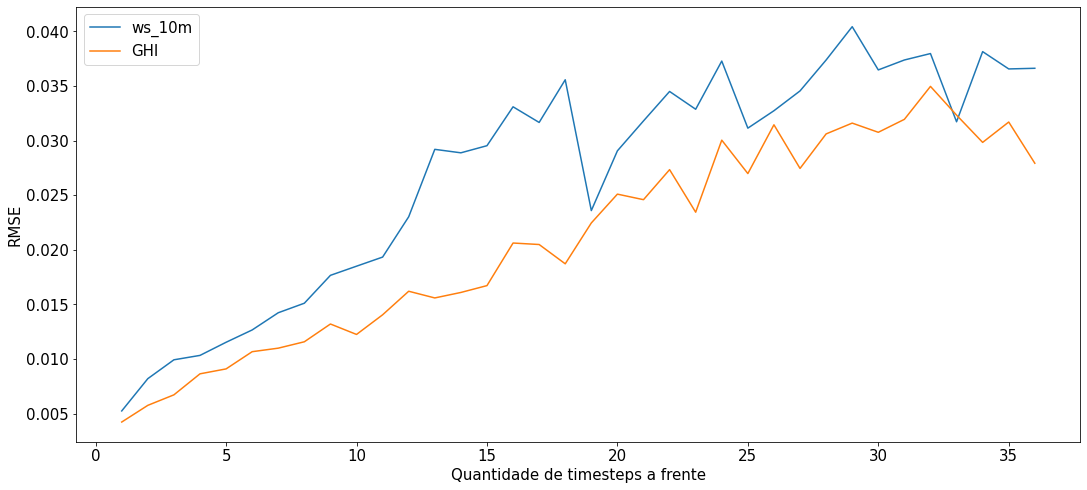
\includegraphics[width=0.8\textwidth]{../img/rmse_last3m.png}
	\caption{\acrshort{rmse} final de cada rede}\label{fig:rmse}
\end{figure}

As previsões da rede eólica inicialmente seguiram os dados mas nas últimas pode
se ver que o comportamento é descaracterizado. O algoritmo aprendeu a prever a
média de forma a reduzir a função custo, como visto na
Figura~\ref{fig:wind:pred}.  A previsão solar teve melhor desempenho, com mais
fidelidade aos dados. Ainda sim, os períodos noturnos provocaram platôs de
inércia, vistos na Figura~\ref{fig:solar:pred18} e~\ref{fig:solar:pred-1}.

% !TEX root = ../0_tcc.tex

\begin{figure}[H]
	\centering
	\begin{subfigure}{\textwidth}
		\centering
		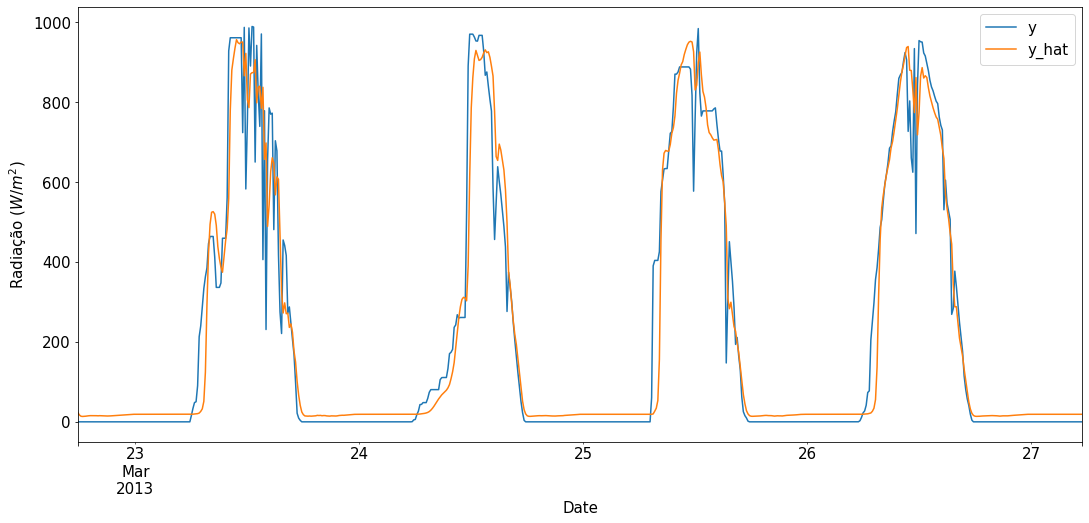
\includegraphics[width=0.7\textwidth]{../img/solar_pred_3m_0.png}
		\caption{Previsão realizada pela primeira rede}\label{fig:solar:pred1}
	\end{subfigure}
	\\ \vspace{1cm}
	\begin{subfigure}{\textwidth}
		\centering
		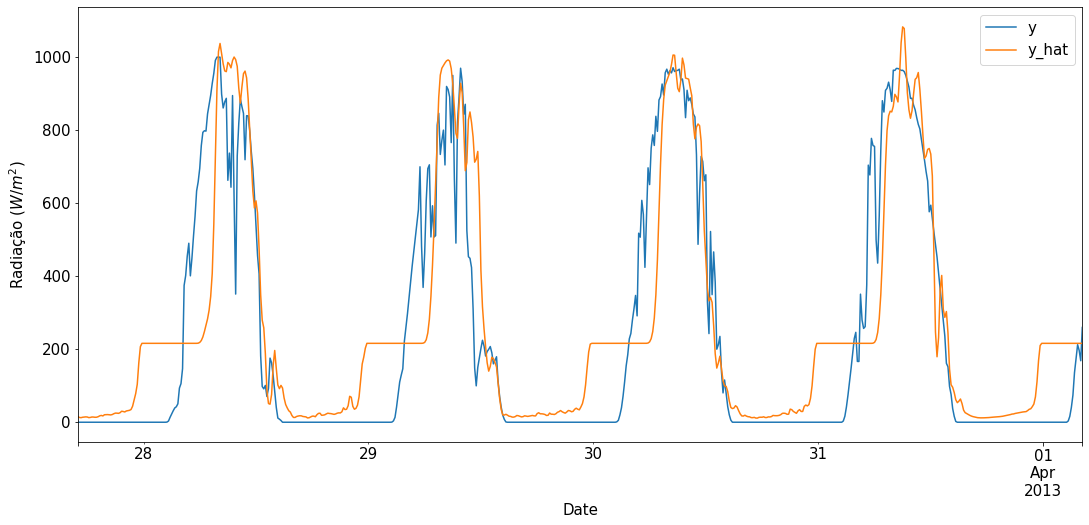
\includegraphics[width=0.7\textwidth]{../img/solar_pred_3m_18.png}
		\caption{Previsão realizada pela décima oitava rede}\label{fig:solar:pred18}
	\end{subfigure}
	\\ \vspace{1cm}
	\begin{subfigure}{\textwidth}
		\centering
		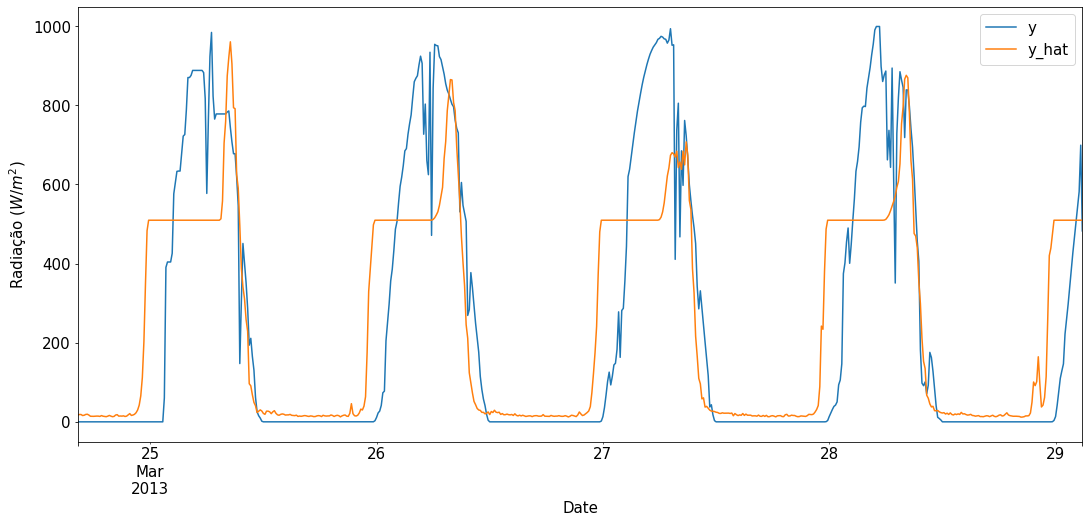
\includegraphics[width=0.7\textwidth]{../img/solar_pred_3m_-1.png}
		\caption{Previsão realizada pela última rede}\label{fig:solar:pred-1}
	\end{subfigure}
	\caption{Previsão de irradiação nos dados de teste}\label{fig:solar:pred}
\end{figure}


% !TEX root = ../00_tcc.tex

\begin{figure}[H]
	\centering
	\begin{subfigure}{\textwidth}
		\centering
		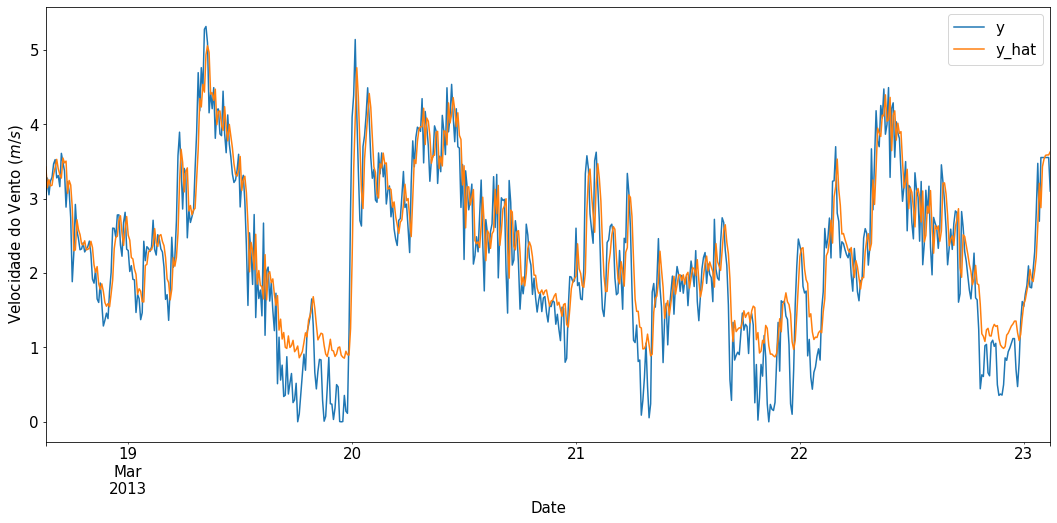
\includegraphics[width=0.7\textwidth]{../img/wind_pred_3m_0.png}
		\caption{Previsão realizada pela primeira rede}\label{fig:wind:pred1}
	\end{subfigure}
	\\ \vspace{1cm}
	\begin{subfigure}{\textwidth}
		\centering
		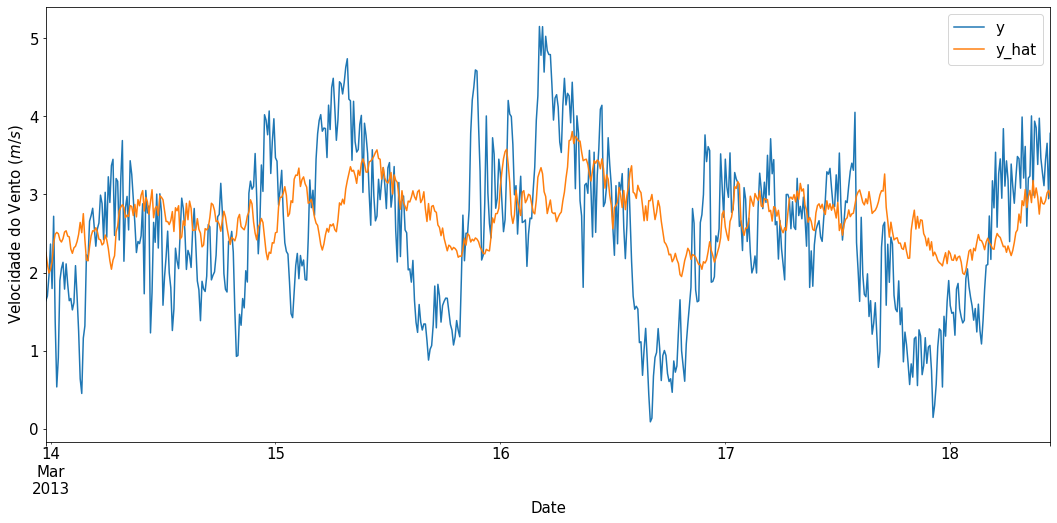
\includegraphics[width=0.7\textwidth]{../img/wind_pred_3m_18.png}
		\caption{Previsão realizada pela décima oitava rede}\label{fig:wind:pred18}
	\end{subfigure}
	\\ \vspace{1cm}
	\begin{subfigure}{\textwidth}
		\centering
		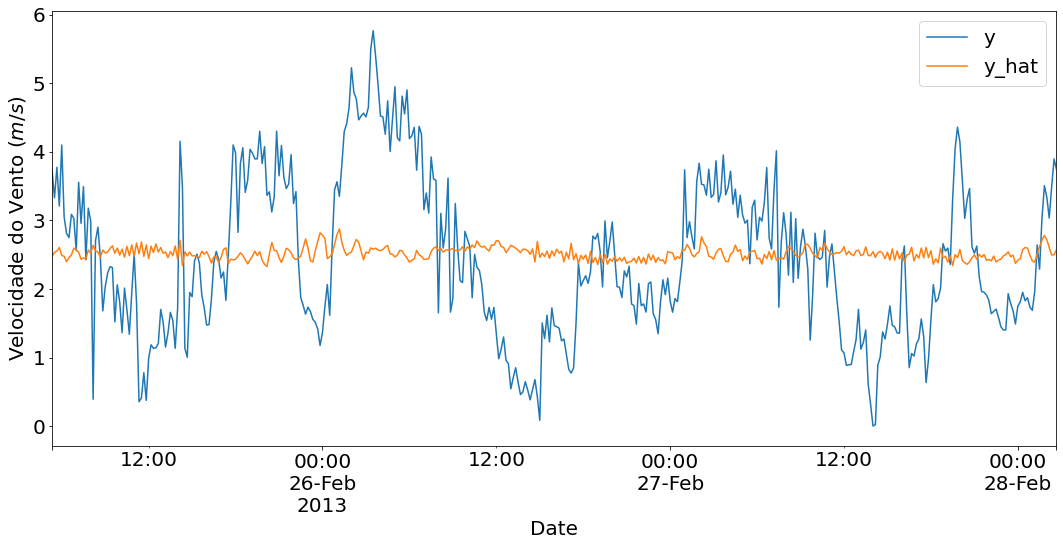
\includegraphics[width=0.7\textwidth]{../img/wind_pred_3m_-1.png}
		\caption{Previsão realizada pela última rede}\label{fig:wind:pred-1}
	\end{subfigure}
	\caption{Previsão de velocidade do vento nos dados de teste}\label{fig:wind:pred}
\end{figure}


Quando aplicadas em conjunto com uma previsão de cada rede, nas
figuras~\ref{fig:solar:comp} e~\ref{fig:wind:comp},  o resultado aparentou
ser satisfatório.

% !TEX root = ../0_tcc.tex

\begin{figure}[H]
	\centering
	\begin{subfigure}{\textwidth}
		\centering
		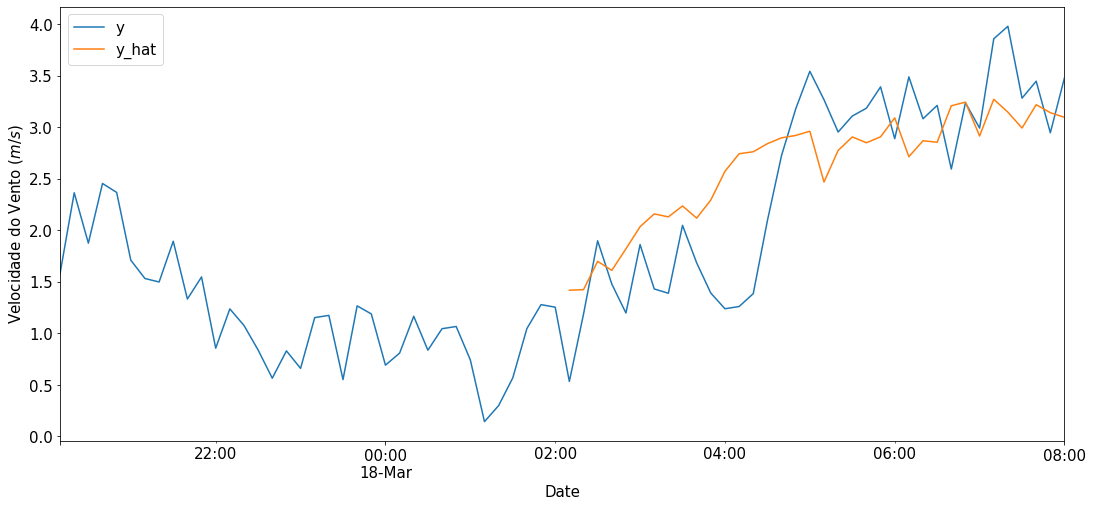
\includegraphics[width=0.8\textwidth]{../img/wind_comp.png}
		\caption{Previsão eólica}\label{fig:wind:comp}
	\end{subfigure}
	\\ \vspace{1cm}
	\begin{subfigure}{\textwidth}
		\centering
		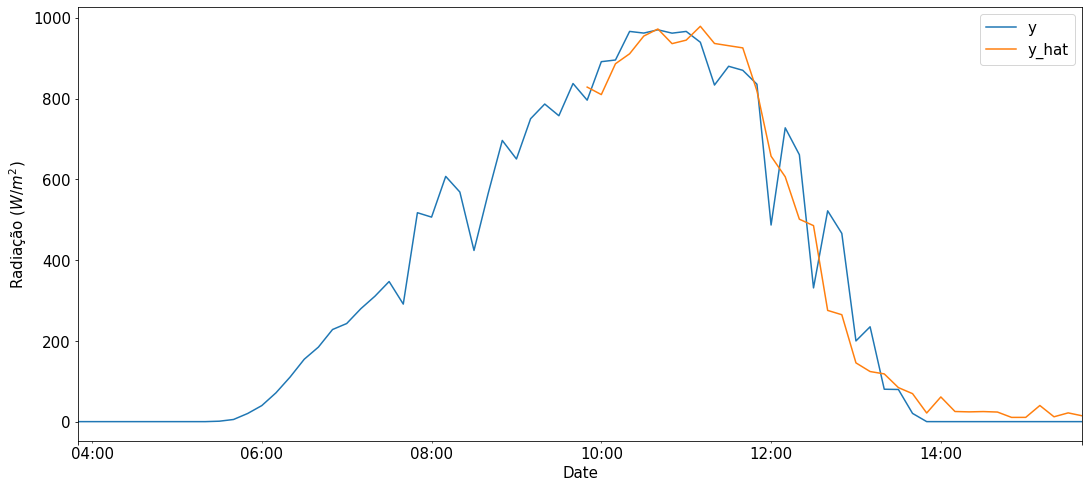
\includegraphics[width=0.8\textwidth]{../img/solar_comp.png}
		\caption{Previsão solar}\label{fig:solar:comp}
	\end{subfigure}
	\caption{Previsão final comparada aos dados reais}\label{fig:comp}
\end{figure}


Com apenas fontes renováveis, o sistema apresentou alto índice de \acrlong{lpsp},
com déficit em 46\% dos instantes de tempo. No cenário de uma única
estratégia de controle para o sistema, a \acrshort{lpsp} caiu consideravelmente.
Diante dessas condições, quando aplicada apenas a estratégia de \acrshort{cc}, é
obtido 5,94\% de \acrshort{lpsp}, já no caso de \acrshort{lf} o percentual é de
7,69\%.

Para mensurar a aplicabilidade de estratégias preditivas, foram feitas previsões
da radiação solar e velocidade do vento para todos intervalos. Em posse das
previsões, métricas foram calculadas em todos os instantes da série temporal.  O
primeiro instante considera a janela de $t$ até $t+36$, o segundo considera
$t+1$ até $t+37$ e assim por diante.  Em cada uma dessas janelas, 4 cenários de
\acrlong{lpsp} foram avaliados: apenas com \acrshort{lf} para dados reais,
apenas com \acrshort{cc} para dados reais e o mesmo para as previsões.  A melhor
estratégia dos dados reais foi comparada com a melhor estratégia prevista pelo
modelo. Caso os resultados fossem iguais, a previsão foi correta.

Inicialmente, o diesel poderia arrancar e parar em qualquer instante, por isso o
comportamento de \acrshort{cc} e \acrshort{lf} foi praticamente o mesmo. Foi
introduzida uma limitação ao grupo diesel de mínimo tempo de execução, uma vez
iniciado. A limitação é comum em máquinas térmicas, com vista a preservar a vida
útil do equipamento. Foram avaliados diferentes valores para o mínimo tempo de
execução.
O estado de carga da bateria exibido na Figura~\ref{fig:soc} ilustra
a diferença de comportamento. Devido à \acrshort{cc} arrancar sempre com maior
potência disponível, a estratégia teve melhor \acrshort{lpsp}.

% !TEX root = ../00_tcc.tex

\begin{figure}[H]
	\centering
	\begin{subfigure}{\textwidth}
		\centering
		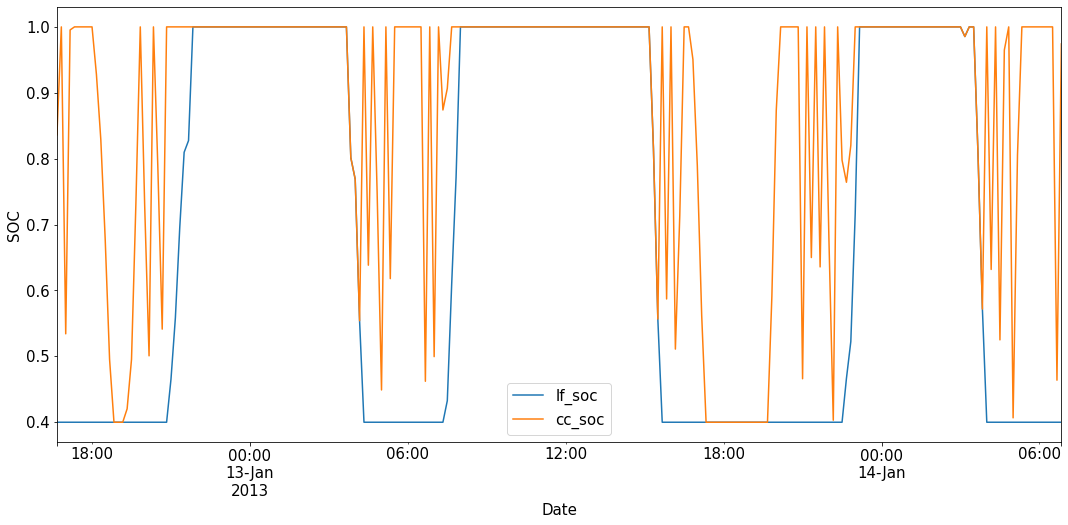
\includegraphics[width=0.7\textwidth]{../img/soc.png}
		\caption{Sem tempo mínimo de funcionamento}\label{fig:soc0}
	\end{subfigure}
	\\ \vspace{1cm}
	\begin{subfigure}{\textwidth}
		\centering
		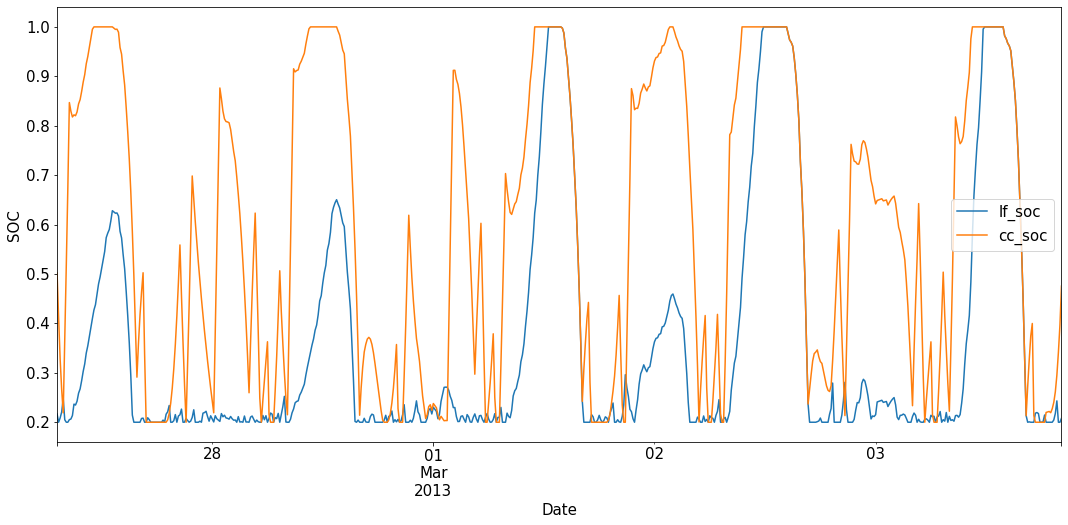
\includegraphics[width=0.7\textwidth]{../img/soc_3.png}
		\caption{Mínima excecução de 3 intervalos}\label{fig:soc3}
	\end{subfigure}
	\\ \vspace{1cm}
	\begin{subfigure}{\textwidth}
		\centering
		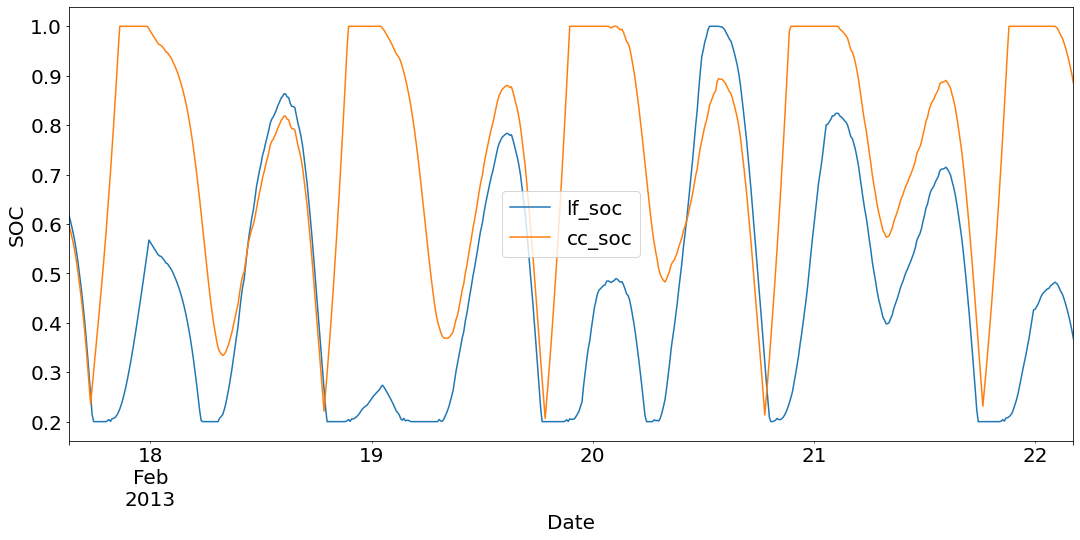
\includegraphics[width=0.7\textwidth]{../img/soc_6.png}
		\caption{Mínima excecução de 6 intervalos}\label{fig:soc6}
	\end{subfigure}
	\caption{Comparação da oscilação do \acrshort{soc}}\label{fig:soc}
\end{figure}


Os resultados para um mínimo tempo do diesel de 6 intervalos foram traçados em
uma matriz de confusão, visto na Figura~\ref{fig:confusion}. As previsões
apresentaram cerca de 75\% de acurácia, tendo previsto
corretamente~\acrshort{lf} como maior \acrshort{lpsp}.

\begin{figure}[H]
	\centering
	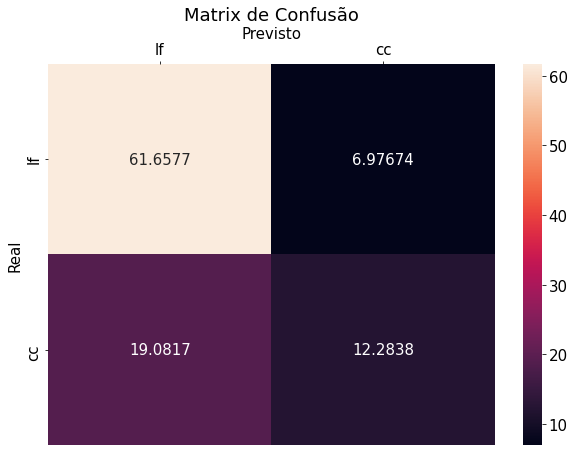
\includegraphics[width=0.6\textwidth]{../img/hm_cc.png}
	\caption{Resultados para previsão}\label{fig:confusion}
\end{figure}

O controle preditivo conseguiu resultados intermediários como exposto na
Tabela~\ref{tbl:comp}.  O comportamento de \acrshort{lpsp} está de acordo com o
estudo de~\cite{das2019performance}, que avalia diferentes estratégias de
controle. No trabalho, é concluído que, no cenário em questão, a maior diferença
entre \acrshort{lf} e \acrshort{cc} é a fração renovável de cada uma e,
consequentemente, o consumo de diesel.

% !TEX root = ../0_tcc.tex

\begin{table}[ht]
	\centering
	\caption{Comparativo de estratégias}\label{tbl:comp}
	\begin{tabular}{lrrr}
		\hline
		                & \acrshort{lf}   & \acrshort{cc} &  \acrshort{lf} e \acrshort{cc} \\
		\hline
		\hline
		\acrshort{lpsp} &  5.94\%         &  7.69\%       &  6.87\%                        \\
		\hline
	\end{tabular}
\end{table}


O \emph{Google Colab} mostrou-se útil para construção e treinamento de modelos
em uma máquina remota.  O uso da ferramenta gratuita pode facilitar
investimentos com pouca disponibilidade de recursos computacionais.As redes
neurais apresentaram baixo \acrshort{rmse}, entretanto previsões de mais longo
prazo mostraram comportamentos errôneos: a solar não previu os picos diários,
compensando em previsões negativas ao fim do dia e a rede eólica seguiu a
tendência mas não acompanhou a amplitude do sinal.  O sistema abastecido apenas
por fontes renováveis apresentou alta probabilidade de perda de carga. Quando
aplicadas as estratégias, tanto \acrshort{lf} quanto \acrshort{cc}, a
\acrshort{lpsp} diminuiu consideravelmente.  Entretanto, o comportamento
preditivo das estratégias foi similar devido à liberdade de arrancar e parar o
gerador diesel a qualquer momento.  Quando introduzido limitações de tempo
mínimo de operação, \acrshort{cc} se tornou a estratégia mais confiável por
causa de sua potência de arranque mais alta.
